\chapter{Code Appendix}

$\textbf{The RMAT Package}$ \hfill \newline

\noindent
The RMAT package is composed of two primary modules, the random matrix module (matrices.R) and the spectral statistics module (spectrum.R) and (dispersion.R). They can be further subdivided into smaller modules as follows.

\begin{enumerate}
  \item \textbf{Random Matrix Module}
    \begin{enumerate}
      \item Explicitly Distributed Matrices
      \item Implicitly Distributed Matrices
      \item Ensemble Extensions
    \end{enumerate}

  \item \textbf{Spectral Statistics Module}
    \begin{enumerate}
      \item Spectrum
      \item Dispersions
      \item Parallel Extensions
      %\item Visualizations
    \end{enumerate}
\end{enumerate}

\newpage

\section{Matrix Module}

\subsection{Explicitly Distributed Matrices}

\subsection{Implicitly Distributed Matrices}

\subsection{Ensemble Extensions}

\newpage

\section{Spectral Statistics Module}

\subsection{Spectrum}

\subsection{Dispersions}

\subsection{Parallel Extensions}


%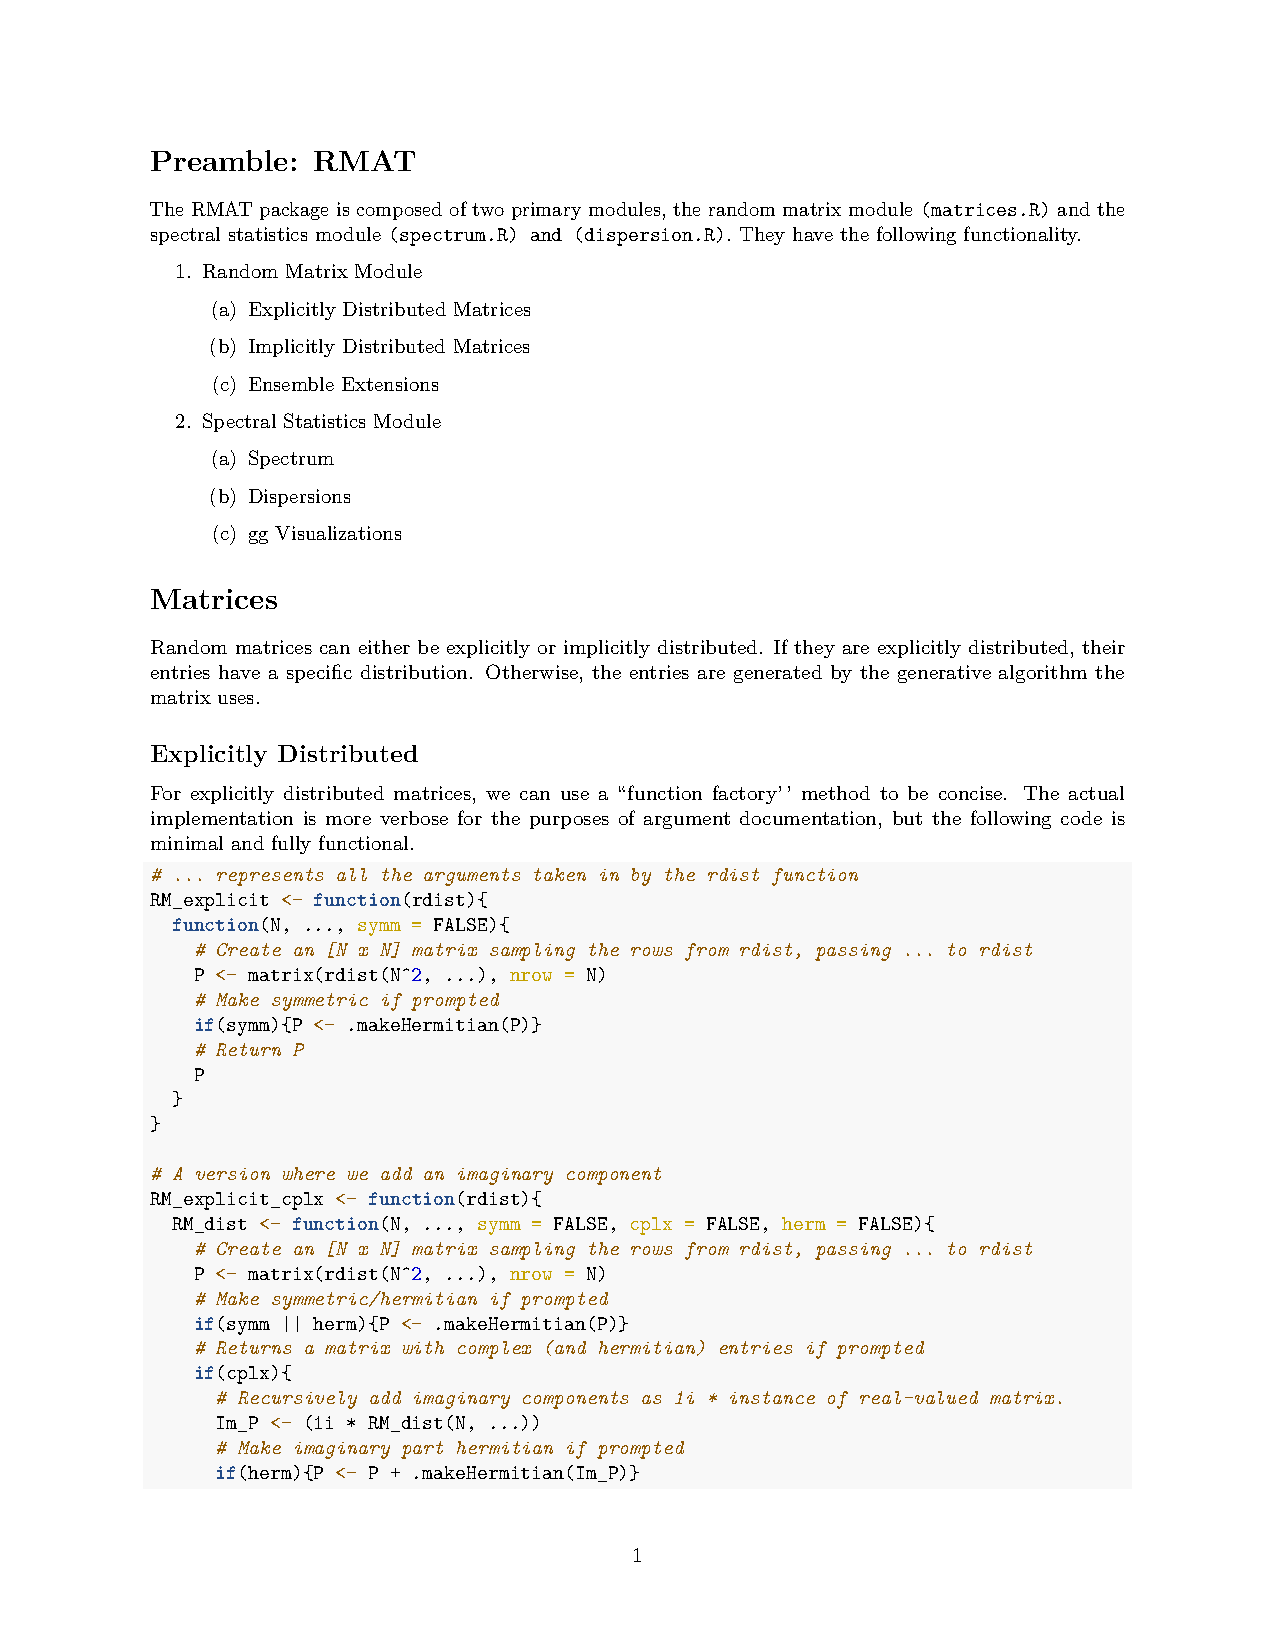
\includepdf[pages=-]{code_appendix_RMD}

% Use \includegraphics!!!!!